\section{Duality}

We know how to solve linear programs by the simplex method. However it is a very complicated algorithm and we would like to generate a certificate that our solution is optimal. Have an example:

\begin{align*}
\min \quad & 7x_1+x_2+5x_3\\
s.t.\quad & x_1 -x_2 +3x_3 \geq 10\\
& 5x_1+2x_2-x_3 \geq 6\\
&x_{1,2,3} \geq 0
\end{align*}

We can easily see than the optimal solution of the LP has to be greater than 10, because the objective function ist strictly greater than the first constraint (and that has to be satisfied in any optimal solution). We can strengthen the observation for example by adding the first two constraints. We get

\[6x_1+x_2+2x_3\geq 16\]

Since the sum of the two constraints has to be satisfied and is still smaller than the objective function, we know that the optimal value has to be greater than 16. Similarly we can first scale one of the rows to calculate tigther lower bounds. 

Systematically we look for $y_1,y_2$ such that $y_1,y_2\geq 0$ and

\[y_1 \cdot \text{1st constraint} + y_2 \cdot \text{2nd constraint} < \text{objective}\]

That means for the above constraints

\begin{align*}
y_1+5y_2 \leq 7\\
-y_1 +2y_2 \leq 1\\
3y_1 - y_2 \leq 5
\end{align*}

Then we get LP $\geq 10y_1 + 6y_2$. If we want to find the optimal values for $y_1$ and $y_2$ we suddenly get a new LP:

\begin{align*}
\max \quad & 10y_1 +6y_2\\
&y_1 + 5y_2 \leq 7\\
&-y_1+2y_2 \leq 1\\
&3y_1 -y_2 \leq 5\\
&y_{1,2} \geq 0
\end{align*}

So to find the optimal value for the lower bound of the old LP, we need to find the optimal value for a new LP. It will turn out, that the optimal value of this LP is actually the same as the optimal value of the old LP. It is its \emph{dual}.

\begin{figure}[hbt]
\begin{center}
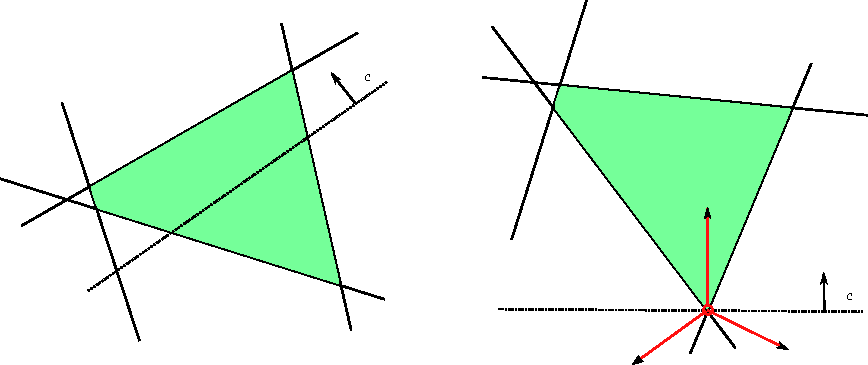
\includegraphics{./images/dual.pdf}
\end{center}
\caption{A balance of forces at the optimal solution}
\label{Fig:ballsOfSteel}
\end{figure}

To get an idea why the dual has the same cost, have a look at figure \ref{Fig:ballsOfSteel}. Suppose we turn the feasible region such as on the right side. The optimal solution $x^*$ is the lowest point. A ball placed in the region will fall to the optimal solution. There a vector pointing in the direction of gravity has to be canceled by the constraints. That means that the objective $c$ has to be canceled by the constraints.

\[\exists y_{b_i}:\ c = \sum_{b_i\in B} y_{b_i} a_{b_i} \Leftrightarrow \trans y A=c \Rightarrow \trans y b = \trans y A x^* = cx^*\]


\begin{Def}[Dual]\label{Def:dual} For an primal LP
\begin{align*}
\min \quad & \sum_j c_j x_j\\
\quad & Ax =b
\end{align*}

We sort the variables and the constraints in three sets, 
\[j \in \begin{cases}
N_1 & x_j\geq 0\\
N_2 & x_j\leq 0\\
N_3 & x_j \text{ free}
\end{cases} \qquad i\in \begin{cases}
M_1 & \trans a_ix \geq b_i\\
M_2 & \trans a_ix \leq b_i\\
M_3 & \trans a_ix = b_i
\end{cases}\]

The dual LP is

\begin{align*}
\max \quad & \sum_i b_iy_i\\
& \trans y A_j \leq c_j & j\in N_1\\
& \trans y A_j \geq c_j & j\in N_2\\
& \trans y A_j = c_j & j\in N_3\\
& y_i \begin{cases}
\geq 0 & i\in M_1\\
\leq 0 & i\in M_2\\
\text{free} & i\in M_3
\end{cases}
\end{align*}

As in the example we introduce a variable $y_i$ for each constraint and one constraint for each variable of the primal LP. We switch the vectors $c$ and $b$
\end{Def}

\begin{thm}[Weak Duality]\label{thm:weakDuality} Given a pair of feasible primal/dual solutions $x,y$
\[cx \geq  \trans b y\]
\end{thm}

\begin{pr} We have

\[y_i(\trans a_ix-b_i) \geq 0 \qquad \forall i\in M_{1,2,3}\]

%explain why

So the sum of those is also positive.

\begin{align*}
\sum_i y_i(\trans a_ix-b_i) &\geq 0\\
(\sum_{i,j}y_ia_{ij}x_j)-\trans yb &\geq 0
\end{align*}

Also 

\begin{align*}
\sum_j x_j(c_j-\trans yA_j) & \geq 0\\
cx - \sum_{i,j} y_i a_{ij} x_j &\geq 0
\end{align*}
%explain why

Hence

\[cx \geq \sum_{i,j} y_i a_{ij} x_j \geq \trans b y\]

But this isn't very surprising because we defined the dual such that this holds.
\end{pr}

\begin{thm}[Strong Duality]\label{thm:strongDuality} If a linear program is feasible and bounded, then so is its dual. The value of the two LPs is the same. \end{thm}

\begin{pr} To make things easier we will just prove it for LPs in standard form.
%TODO side by side
\begin{align*}
\min \quad & cx\\
& Ax = b\\
&x\geq 0
\end{align*}

\begin{align*}
\max \quad &\trans by\\
& \trans yA \leq c\\
& y \text{ free}
\end{align*}

By running simplex on the primal we get an optimal basis $B$. If simplex returned that basis, the reduced costs for that basis were all $\geq 0$

\begin{align*}
c-c_BA_B^{-1}A &\geq 0\\
c \geq \underbrace{c_BA_B^{-1}}_{:=\trans y}A
\end{align*}

From that we see that $\trans y$ is a feasible dual solution. We need to show that the cost for this solution is at least as good as the cost of the primal solution. Then by theorem \ref{thm:weakDuality} the optimal costs for both LPs must be the same.

So let's look at the cost of the dual solution $\trans y b$. Because $B$ is a feasible basis, it introduces a bfs $x$. We have

\begin{align*}
b &= Ax\\
\trans y b &= \trans y A x\\
 &=\trans y A_B x_B\\
 &=c_B A_B^{-1}A_B x_B\\
 &=c_B x_B
 \end{align*}
 
 For LPs which are not in standard form we first transform the primal into normal form. Some similar transformation is done on the dual. Then you prove that the transformed LPs have the same optimal value.
\end{pr}

A nice consequence of this theorem is an easy way to show that primal and dual solutions are optimal.

\begin{thm}[Complementary Slackness] Let $x$ and $y$ be a pair of feasible primal-dual solutions. Then $x$ \emph{and} $y$ are optimal iff
\begin{align*}
y_i(\trans A_ix-b_i) = 0 && \forall i\\ 
(c_j - \trans yA_j)x_j =0 && \forall j
\end{align*}
\end{thm}

\begin{pr}\mbox{}\\
\begin{itemize}
\item[$\Leftarrow$] That follows from the proof of theorem \ref{thm:weakDuality} (replace $\leq 0$ by $=0$)
\item[$\Rightarrow$] %TODO also follows from weakDuality proof. You get strict inequalities.
\end{itemize}
\end{pr}

When we run the simplex algorithm we have three possible answers. Let's see how they relate 

\begin{center}
\begin{tabular}{lc|ccc|}\cline{3-5}
    & & \multicolumn{3}{c|}{Dual}\\\cline{3-5}
   &  & Feasible Bounded & Feasible Unbounded & Not Feasible\\\hline
\multicolumn{1}{|c}{\multirow{3}{*}{\begin{sideways}Primal\end{sideways}}}& \multicolumn{1}{|c|}{Feasible, Bounded} & \ok  & \no  & \no   \\
\multicolumn{1}{|c}{}&\multicolumn{1}{|c|}{Feasible, Unbounded} & \no &  \no & \ok  \\
\multicolumn{1}{|c}{}&\multicolumn{1}{|c|}{Not Feasible} &  \no  & \ok  & \ok  \\\hline
\end{tabular}
\end{center}

The Unbounded --- Not Feasible result follows from weak duality. If one is unbounded there can't be any solution for the other, because the inequality of theorem \ref{thm:weakDuality} would put a bound on the value.

\begin{Ex}[Max-Flow] We already saw the LP for the maximum flow problem and its dual the min cut LP in the first lecture. See example \ref{Ex:maxFlowMinCut}. We have variables $c_{uv} \geq x_{uv}\geq 0$ for each edge $(u,v)$ in the graph where  $c_{uv}$ is the capacity. Also we have the flow conservation constraints.

%TODO wo zaubert der diese nummerierung her?
\begin{align}
\max \quad & \sum_{u\in V} x_{su}\\
&\sum_{u\in V} x_{uv} - \sum_{u\in V} x_{vu} = 0 && \forall v \neq s,t \label{maxFlow1}\\
&x_{uv} \leq c_{uv}	&& \forall (u,v)\in E\label{maxFlow2}\\
&x_{uv} \geq 0 && \forall (u,v)\in E
\end{align}

We construct the dual problem by associating a variable $\alpha_v$ for each constraint from \ref{maxFlow1} and $\beta_{uv}$ for each constraint from \ref{maxFlow2}. By looking at the definition \ref{Def:dual} we can see how the constraints have to be constructed.

\begin{align}
\min \quad & \sum c_{uv}\beta_{uv}\\
 & -\alpha_u + \alpha_v  + \beta_{uv} \geq 0 && \forall (u,v): u,v\neq s,t\label{mincut1}\\
 & \alpha_v + \beta_{uv} \geq 1 && \forall (s,v)\label{mincut2}\\
 & -\alpha_u + \beta_{uv} \geq 0 && \forall(u,t)\label{mincut3}\\
 & \alpha_v \text{ free}\\
 & \beta_{uv} \geq 0
\end{align}

Line \ref{mincut1} is for variables $x_{uv}$, line \ref{mincut2} is for variables $x_{sv}$ and line \ref{mincut3} is for variables $x_{ut}$. 

Lets do some observations on the new LP: 

\begin{itemize}
\item We can rewrite the constraints in \ref{mincut1} like this

\[\alpha_u \leq \alpha_v + \beta_{uv}\]

\item Even though the $\alpha_v$ are free, there is no point in making them negative. 
\item Similarly the $\alpha_v$ are less than 1.
\item We could introduce two new variables with $\alpha_s=1$, $\alpha_t=0$.
\end{itemize}

The LP separates graph in two components, one where the $\alpha$ are 1 and those where the $\alpha$ are 0. On the edges that cross that cut the $\beta$ have to be 1. %look at the constraints and explain why
\end{Ex}